%% bare_conf.tex
%% V1.4b
%% 2015/08/26
%% by Michael Shell
%% See:
%% http://www.michaelshell.org/
%% for current contact information.
%%
%% This is a skeleton file demonstrating the use of IEEEtran.cls
%% (requires IEEEtran.cls version 1.8b or later) with an IEEE
%% conference paper.
%%
%% Support sites:
%% http://www.michaelshell.org/tex/ieeetran/
%% http://www.ctan.org/pkg/ieeetran
%% and
%% http://www.ieee.org/

%%*************************************************************************
%% Legal Notice:
%% This code is offered as-is without any warranty either expressed or
%% implied; without even the implied warranty of MERCHANTABILITY or
%% FITNESS FOR A PARTICULAR PURPOSE! 
%% User assumes all risk.
%% In no event shall the IEEE or any contributor to this code be liable for
%% any damages or losses, including, but not limited to, incidental,
%% consequential, or any other damages, resulting from the use or misuse
%% of any information contained here.
%%
%% All comments are the opinions of their respective authors and are not
%% necessarily endorsed by the IEEE.
%%
%% This work is distributed under the LaTeX Project Public License (LPPL)
%% ( http://www.latex-project.org/ ) version 1.3, and may be freely used,
%% distributed and modified. A copy of the LPPL, version 1.3, is included
%% in the base LaTeX documentation of all distributions of LaTeX released
%% 2003/12/01 or later.
%% Retain all contribution notices and credits.
%% ** Modified files should be clearly indicated as such, including  **
%% ** renaming them and changing author support contact information. **
%%*************************************************************************


% *** Authors should verify (and, if needed, correct) their LaTeX system  ***
% *** with the testflow diagnostic prior to trusting their LaTeX platform ***
% *** with production work. The IEEE's font choices and paper sizes can   ***
% *** trigger bugs that do not appear when using other class files.       ***                          ***
% The testflow support page is at:
% http://www.michaelshell.org/tex/testflow/



\documentclass[conference]{IEEEtran}
% Some Computer Society conferences also require the compsoc mode option,
% but others use the standard conference format.
%
% If IEEEtran.cls has not been installed into the LaTeX system files,
% manually specify the path to it like:
% \documentclass[conference]{../sty/IEEEtran}





% Some very useful LaTeX packages include:
% (uncomment the ones you want to load)


% *** MISC UTILITY PACKAGES ***
%
%\usepackage{ifpdf}
% Heiko Oberdiek's ifpdf.sty is very useful if you need conditional
% compilation based on whether the output is pdf or dvi.
% usage:
% \ifpdf
%   % pdf code
% \else
%   % dvi code
% \fi
% The latest version of ifpdf.sty can be obtained from:
% http://www.ctan.org/pkg/ifpdf
% Also, note that IEEEtran.cls V1.7 and later provides a builtin
% \ifCLASSINFOpdf conditional that works the same way.
% When switching from latex to pdflatex and vice-versa, the compiler may
% have to be run twice to clear warning/error messages.






% *** CITATION PACKAGES ***
%
%\usepackage{cite}
% cite.sty was written by Donald Arseneau
% V1.6 and later of IEEEtran pre-defines the format of the cite.sty package
% \cite{} output to follow that of the IEEE. Loading the cite package will
% result in citation numbers being automatically sorted and properly
% "compressed/ranged". e.g., [1], [9], [2], [7], [5], [6] without using
% cite.sty will become [1], [2], [5]--[7], [9] using cite.sty. cite.sty's
% \cite will automatically add leading space, if needed. Use cite.sty's
% noadjust option (cite.sty V3.8 and later) if you want to turn this off
% such as if a citation ever needs to be enclosed in parenthesis.
% cite.sty is already installed on most LaTeX systems. Be sure and use
% version 5.0 (2009-03-20) and later if using hyperref.sty.
% The latest version can be obtained at:
% http://www.ctan.org/pkg/cite
% The documentation is contained in the cite.sty file itself.






% *** GRAPHICS RELATED PACKAGES ***
%
\ifCLASSINFOpdf
  \usepackage[pdftex]{graphicx}
  % declare the path(s) where your graphic files are
  \graphicspath{{images/}}
  % and their extensions so you won't have to specify these with
  % every instance of \includegraphics
  \DeclareGraphicsExtensions{.pdf}
\else
  % or other class option (dvipsone, dvipdf, if not using dvips). graphicx
  % will default to the driver specified in the system graphics.cfg if no
  % driver is specified.
  % \usepackage[dvips]{graphicx}
  % declare the path(s) where your graphic files are
  % \graphicspath{{../eps/}}
  % and their extensions so you won't have to specify these with
  % every instance of \includegraphics
  % \DeclareGraphicsExtensions{.eps}
\fi
% graphicx was written by David Carlisle and Sebastian Rahtz. It is
% required if you want graphics, photos, etc. graphicx.sty is already
% installed on most LaTeX systems. The latest version and documentation
% can be obtained at: 
% http://www.ctan.org/pkg/graphicx
% Another good source of documentation is "Using Imported Graphics in
% LaTeX2e" by Keith Reckdahl which can be found at:
% http://www.ctan.org/pkg/epslatex
%
% latex, and pdflatex in dvi mode, support graphics in encapsulated
% postscript (.eps) format. pdflatex in pdf mode supports graphics
% in .pdf, .jpeg, .png and .mps (metapost) formats. Users should ensure
% that all non-photo figures use a vector format (.eps, .pdf, .mps) and
% not a bitmapped formats (.jpeg, .png). The IEEE frowns on bitmapped formats
% which can result in "jaggedy"/blurry rendering of lines and letters as
% well as large increases in file sizes.
%
% You can find documentation about the pdfTeX application at:
% http://www.tug.org/applications/pdftex





% *** MATH PACKAGES ***
%
%\usepackage{amsmath}
% A popular package from the American Mathematical Society that provides
% many useful and powerful commands for dealing with mathematics.
%
% Note that the amsmath package sets \interdisplaylinepenalty to 10000
% thus preventing page breaks from occurring within multiline equations. Use:
%\interdisplaylinepenalty=2500
% after loading amsmath to restore such page breaks as IEEEtran.cls normally
% does. amsmath.sty is already installed on most LaTeX systems. The latest
% version and documentation can be obtained at:
% http://www.ctan.org/pkg/amsmath





% *** SPECIALIZED LIST PACKAGES ***
%
%\usepackage{algorithmic}
% algorithmic.sty was written by Peter Williams and Rogerio Brito.
% This package provides an algorithmic environment fo describing algorithms.
% You can use the algorithmic environment in-text or within a figure
% environment to provide for a floating algorithm. Do NOT use the algorithm
% floating environment provided by algorithm.sty (by the same authors) or
% algorithm2e.sty (by Christophe Fiorio) as the IEEE does not use dedicated
% algorithm float types and packages that provide these will not provide
% correct IEEE style captions. The latest version and documentation of
% algorithmic.sty can be obtained at:
% http://www.ctan.org/pkg/algorithms
% Also of interest may be the (relatively newer and more customizable)
% algorithmicx.sty package by Szasz Janos:
% http://www.ctan.org/pkg/algorithmicx




% *** ALIGNMENT PACKAGES ***
%
%\usepackage{array}
% Frank Mittelbach's and David Carlisle's array.sty patches and improves
% the standard LaTeX2e array and tabular environments to provide better
% appearance and additional user controls. As the default LaTeX2e table
% generation code is lacking to the point of almost being broken with
% respect to the quality of the end results, all users are strongly
% advised to use an enhanced (at the very least that provided by array.sty)
% set of table tools. array.sty is already installed on most systems. The
% latest version and documentation can be obtained at:
% http://www.ctan.org/pkg/array


% IEEEtran contains the IEEEeqnarray family of commands that can be used to
% generate multiline equations as well as matrices, tables, etc., of high
% quality.




% *** SUBFIGURE PACKAGES ***
%\ifCLASSOPTIONcompsoc
%  \usepackage[caption=false,font=normalsize,labelfont=sf,textfont=sf]{subfig}
%\else
%  \usepackage[caption=false,font=footnotesize]{subfig}
%\fi
% subfig.sty, written by Steven Douglas Cochran, is the modern replacement
% for subfigure.sty, the latter of which is no longer maintained and is
% incompatible with some LaTeX packages including fixltx2e. However,
% subfig.sty requires and automatically loads Axel Sommerfeldt's caption.sty
% which will override IEEEtran.cls' handling of captions and this will result
% in non-IEEE style figure/table captions. To prevent this problem, be sure
% and invoke subfig.sty's "caption=false" package option (available since
% subfig.sty version 1.3, 2005/06/28) as this is will preserve IEEEtran.cls
% handling of captions.
% Note that the Computer Society format requires a larger sans serif font
% than the serif footnote size font used in traditional IEEE formatting
% and thus the need to invoke different subfig.sty package options depending
% on whether compsoc mode has been enabled.
%
% The latest version and documentation of subfig.sty can be obtained at:
% http://www.ctan.org/pkg/subfig




% *** FLOAT PACKAGES ***
%
%\usepackage{fixltx2e}
% fixltx2e, the successor to the earlier fix2col.sty, was written by
% Frank Mittelbach and David Carlisle. This package corrects a few problems
% in the LaTeX2e kernel, the most notable of which is that in current
% LaTeX2e releases, the ordering of single and double column floats is not
% guaranteed to be preserved. Thus, an unpatched LaTeX2e can allow a
% single column figure to be placed prior to an earlier double column
% figure.
% Be aware that LaTeX2e kernels dated 2015 and later have fixltx2e.sty's
% corrections already built into the system in which case a warning will
% be issued if an attempt is made to load fixltx2e.sty as it is no longer
% needed.
% The latest version and documentation can be found at:
% http://www.ctan.org/pkg/fixltx2e


%\usepackage{stfloats}
% stfloats.sty was written by Sigitas Tolusis. This package gives LaTeX2e
% the ability to do double column floats at the bottom of the page as well
% as the top. (e.g., "\begin{figure*}[!b]" is not normally possible in
% LaTeX2e). It also provides a command:
%\fnbelowfloat
% to enable the placement of footnotes below bottom floats (the standard
% LaTeX2e kernel puts them above bottom floats). This is an invasive package
% which rewrites many portions of the LaTeX2e float routines. It may not work
% with other packages that modify the LaTeX2e float routines. The latest
% version and documentation can be obtained at:
% http://www.ctan.org/pkg/stfloats
% Do not use the stfloats baselinefloat ability as the IEEE does not allow
% \baselineskip to stretch. Authors submitting work to the IEEE should note
% that the IEEE rarely uses double column equations and that authors should try
% to avoid such use. Do not be tempted to use the cuted.sty or midfloat.sty
% packages (also by Sigitas Tolusis) as the IEEE does not format its papers in
% such ways.
% Do not attempt to use stfloats with fixltx2e as they are incompatible.
% Instead, use Morten Hogholm'a dblfloatfix which combines the features
% of both fixltx2e and stfloats:
%
% \usepackage{dblfloatfix}
% The latest version can be found at:
% http://www.ctan.org/pkg/dblfloatfix




% *** PDF, URL AND HYPERLINK PACKAGES ***
%
%\usepackage{url}
% url.sty was written by Donald Arseneau. It provides better support for
% handling and breaking URLs. url.sty is already installed on most LaTeX
% systems. The latest version and documentation can be obtained at:
% http://www.ctan.org/pkg/url
% Basically, \url{my_url_here}.




% *** Do not adjust lengths that control margins, column widths, etc. ***
% *** Do not use packages that alter fonts (such as pslatex).         ***
% There should be no need to do such things with IEEEtran.cls V1.6 and later.
% (Unless specifically asked to do so by the journal or conference you plan
% to submit to, of course. )

\usepackage{glossaries}

\newacronym{mdse}{MDSE}{Model-driven software engineering}
\newacronym{bpmn}{BPMN}{Business Process Modelling Notation}
\newacronym{ct}{CT}{category theory}
\newacronym{uml}{UML}{Unified Modelling Language}
\newacronym{dsl}{DSL}{Domain Specific Language}
\newacronym{csp}{CSP}{Communication Sequential Processes}

% correct bad hyphenation here
\hyphenation{be-ha-vi-o-ral}


\begin{document}
\title{Integrating behavioral models\\ into multi modelling}

\author{\IEEEauthorblockN{Tim Kräuter}
\IEEEauthorblockA{Høgskulen på Vestlandet\\
Bergen, Norway\\
Email: tkra@hvl.no}}


\maketitle

% As a general rule, do not put math, special symbols or citations
% in the abstract
\begin{abstract}
Behavioral models play an important role in \gls{mdse}.
Keeping inter-related behavioral models consistent is essential to use them in \gls{mdse} successfully. 
However, consistency checking for behavioral models, especially in a heterogeneous scenario, is limited.

In this paper, I propose a framework to integrate heterogeneous behavioral modeling languages such that consistency checking can be achieved in broader scenarios.
It is based on aligning the respective behavioral metamodels by defining possible inter-model relations which carry behavioral meaning.
Converting the models together with their relations to a behavioral formalism enables analysis of behavioral consistency using model-checking. 
\end{abstract}

% no keywords

\IEEEpeerreviewmaketitle



\section{Problem}
A significant motivation for \gls{mdse} is to handle the increasing complexity of software systems by a clear separation of concerns \cite{franceModeldrivenDevelopmentComplex2007}.
In the multi-view modelling approach a set of models is developed for the different aspect of a system.
It is often the case that separate groups of people works independently on the aspects of the system.
However, this separation of concerns causes problems because models must be kept consistent with each other, i.e., they should not contain contradicting information \cite{cicchettiMultiviewApproachesSoftware2019}.
% MDSE will fail if the underlying models are inconsistent!
Without this inter-model consistency \gls{mdse} cannot deliver on the promised increased productivity and reduction of errors \cite{brambillaModeldrivenSoftwareEngineering2017}.

% MDSE is heterogeneous and has to be kept consistent.
This is especially problematic when the used models are heterogeneous.
Firstly, there exist structural models such as class diagrams and entity-relationship diagrams.
Secondly, behavioral diagrams are used to describe the dynamics of a system.
Widely used diagrams or formalisms for specifying behavior are state machines, activity diagrams, Petri nets and process algebras.

% We already deal with structural models/ consistency
Inter-model consistency for structural models has been researched extensively.
One promising approach is model weaving \cite{bezivinCanonicalSchemeModel2006}, which establishes links between models with the goal of automatic consistency checking.
Typically, these inter-relations focus on structural aspects, such as identity, usage, dependency, refinement, etc. \cite{feldmannManagingIntermodelInconsistencies2019, torresSystematicLiteratureReview2020}.
They are called \textit{correspondences} on the metamodel level and \textit{commonalities} on the model level \cite{stunkelMultipleModelSynchronization2020, klareCommonalitiesPreservingConsistency2019}.
Inter-model constraints can then be defined and automatically checked on a global model obtained by using the commonalities to merge individual models \cite{stunkelMultimodelCorrespondenceIntermodel2018} or establish a comprehensive view of the overall model \cite{stunkelMultipleModelSynchronization2020}.

% We have to deal with behavioral/semantic consistency between behavioral models especially of heterogeneous nature
However, there is no general approach to check behavioral consistency sometimes also called semantic consistency.
Two behavioral models describing two interacting parts of a system should be checked for deadlocks, live-locks or other system specific aspects.
If the two models conform to the same formalisms or modeling language this is generally not a problem.
But in a heterogeneous case one still wants to define interactions between the models and check behavioral consistency.

Only using one formalism or modeling language for behavioral models is not feasible since one wants to use the most suitable formalism or modeling language in a given situation.
The modeling formalisms used in a given situation depends on the system requirements, existing software landscape and the knowledge, as well as preferences of the responsible developers. 

% We have to deal with consistency between structural and behavioral models in the future as well. Since structural models are graphs, graph transformations seem promising to integrate this in the future.
There can also be consistency rules spanning structural and behavioral models.
For example messages to objects in a \gls{uml} sequence diagram have to match the corresponding classes methods in an class diagram \cite{egyedFixingInconsistenciesUML2007}.
I will focus on behavioral consistency before addressing consistency between structural and behavioral models in the future. 
\section{Related work}
% Engels
In \cite{engelsMethodologySpecifyingAnalyzing2001} they work on consistency of object-oriented behavioral models formulated as capsule state charts in \gls{uml}-RT.
% They are restricted to UML behavioral models --> homo case
Consequently, they are dealing with a homogeneous modeling environment where all behavioral models are formulated in the same modeling language.
The authors use the term semantic consistency instead of behavioral consistency.
To check behavioral consistency they map state chart models to \gls{csp}.
Using the well-defined semantics of \gls{csp} they validate deadlock freeness and the processes compliance to a previously defined communication protocol.
Their proposed general methodology to analyze consistency is to find a suitable semantic domain and map the models into it.
The semantic domain can then be exploited to check consistency.

Based on this methodology consistency checking for sequence diagrams and state charts was developed in \cite{kusterExplicitBehavioralConsistency2003}.
The consistency requirement is that all possible interactions specified within sequence diagrams for each class should be possible regarding the behavior of that class specified in a state chart.
As a semantic domain the authors have successfully used \gls{csp} again.

Besides process algebras such as \gls{csp} different types of petri nets are used for behavioral consistency checking.
In \cite{yaoConsistencyCheckingUML2006} petri nets were used to check consistency for sequence diagrams and state charts.
\cite{cunhaFormalVerificationUML2011} analyses sequence diagrams in the context of embedded systems using a transformation to petri nets.
Consistency for \gls{uml} activity diagrams was checked using petri nets in \cite{thierry-miegUMLBehavioralConsistency2008}.

All the approaches use model checking to analyze behavioral consistency and follow the methodology defined in \cite{engelsMethodologySpecifyingAnalyzing2001} with variations in the semantic domain.
However, the approaches cover only homogeneous scenarios where all models conform to one modeling language.
An exception is the consistency checking between sequence diagrams and state charts.
In practice one could encounter a situation where for example the combination of state machines, process algebras, petri nets and activity diagrams is desired\footnote{The merger of two companies and their IT-infrastructure could for example cause strong heterogeneity in the used modeling languages.}.
Using our proposed approach it is possible to check behavioral consistency even in heterogeneous modeling scenarios.
This leads to more freedom of choice regarding behavioral modeling and model combinations.
In addition, behavioral models of higher quality can be achieved which lay the foundation for successful and effective \gls{mdse}.

\section{Proposed solution}
% this basically extends the methodology presented in the engels paper. Maybe we should write that
The proposed solution extends the methodology presented in \cite{engelsMethodologySpecifyingAnalyzing2001} by incorporating a new step from the multi-model consistency management process targeted towards structural models defined in \cite{stunkelMultipleModelSynchronization2020}.
The proposed solution can be summarized in the four-step process in Figure \ref{fig:consistency_process} and will now  be explained in detail.

\begin{figure}[!t]
\centering
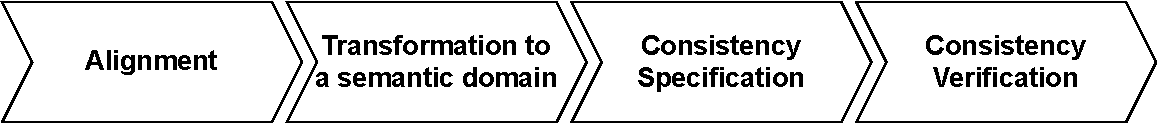
\includegraphics[width=3.4in]{methodology}
\caption{Behavioral Consistency Management Process}
\label{fig:consistency_process}
\end{figure}

% 1. Metamodel and model aligment
To check inter-model consistency for structural models one defines inter-relations between models on the meta-model level and on the model level to describe overlaps in information \cite{stunkelMultipleModelSynchronization2020}.
I propose a similar approach for behavioral models based on inter-model relations.
The inter-model relations should define how behavioral models coordinate which leads to the behavior of the composite system consisting of all individual models.

First one has to define which inter-model relations are allowed.
I will accomplish this by model-weaving on the metamodel-level, i.e. defining a metamodel for the inter-model relations.
This is also called \textit{metamodel alignment} and is a key activity in the multi-model consistency management process \cite{stunkelMultipleModelSynchronization2020}.
For this approach to work, there has to be a metamodel for used model.
However, developing a metamodel if it is not already present is a one-time expense.
Similarly metamodel alignment has to be only done once.
In section \ref{sec:currentStatus} we will align the metamodels for state machines, petri nets and the $\pi$-calculus.
In the future other formalisms can be integrated in a similar way.
After aligning the metamodels one can define inter-model relations between the behavioral models, i.e. align the models.
For example, the synchronisation of a transition in a state machine with a transition in a petri net could be specified.

% 2. Transformation to a semantic domain (proposes graph grammars)
The second activity in the process is to transform the models into a suitable semantic domain respecting their inter-model relations.
By including the inter-model relations in the transformation we can deal with a heterogeneous modeling scenario compared to the original methodology in \cite{engelsMethodologySpecifyingAnalyzing2001}.
A feasible approach is to translate each model individually and then combine them according to the defined inter-model relations.

We will use graph grammars as a behavioral formalism for the models (see section \ref{sec:currentStatus}) because of the following reasons.
Many behavioral formalism have been described by graph grammars for example state machines \cite{kuskeFormalSemanticsUML2001, varroFormalSemanticsUML2002}, petri nets \cite{ehrigGraphGrammarsPetri2004} and the $\pi$-calculus \cite{gadducciGraphRewritingPcalculus2007}.
By using graph grammars one stays on a higher level of abstraction compared to for example transitions systems as a semantic domain.
This has the advantage that the state space generated by graph grammars is better understandable.
I hope that counter examples for consistency constraints will be easier to understand because using graph grammars we stay closer to the original modeling formalisms.
In addition, structural models are formalized as graphs or graph-like structures \cite{stunkelMultipleModelSynchronization2020}, which can lead to an integration of behavioral and structural models using graph transformations in the future. 

However, the semantic domain is interchangeable as long as there is an interpretation for the given models and their inter-relations.

% 3. Consistency specification in some temporal logic
%. 4. Consistency Verification
The third and forth step in the process are concerned with specifying and verifying behavioral consistency.
We assume there is a set of atomic propositions for each model, such that we can calculate their disjoint union.
The semantic domain should generate a state space for the overall system which can be connected to the original models to reattach the atomic propositions.
Finally, one gets a Kripke structure to check behavioral constraints on.
In the best case the specification of constraints is independent of the semantic domain choice.
Besides checking general properties such as deadlocks or simple safety properties, users must be able to define more complex properties in a temporal logic.
I aim to reuse existing model checkers for evaluating these formulas on the calculated Kripke structure.
\section{Plan for evaluation and validation}
% Design science? --> Develop prototype to execute the combined model.
% Evaluate using examples/case studies (hopefully from practice). Check performance

\section{Expected contributions}
% Relating behavioral models (aligning the respective metamodels)
% Semantics as a basis for behavioral consistency.
% Advancement in behavioral/semantic consistency for more consistent models.
\section{Current status} \label{sec:currentStatus}
% Example GG for FSM's, petri-nets and CCS/pi-calculus (process algebra representative).
% (Activity diagrams and bpmn could also be interesting).
% Gets complicated if the behavioral models get too detailed/ too expressive for graph transformations. We need to stay on a high level of abstraction
% Align metamodels
% Running example
% Constraint check on the generated state space.

% Future work or limitations.
% State space generation fast enough? --> Tricks using the underlying models to match rules.
% How to describe colored petri nets or other more complex models?

% Discuss the drawbacks. Slow state space generation? Performance?
% High level modelling. Not on the level of detail for which we would need colored petri nets and more sophisitcated kinds of automata (to express these details in a straight forward way).

\section{Conclusion}
The conclusion goes here.

\section*{Acknowledgment}
The authors would like to thank...

\bibliographystyle{IEEEtran}
\bibliography{bib}

\end{document}


